% Author: Daniel Vartanian
% Version: 0.0.0.9000 2025-03-11
% Licence: The LaTeX Project Public License 1.3c.
%   See <http://www.latex-project.org/lppl.txt> to learn more.
% Note: Run with LuaLaTeX.

% -----
% Preamble
% -----

% ----- Option Settings -----

\PassOptionsToPackage{
  unicode,
  bookmarksnumbered
}{hyperref}

\PassOptionsToPackage{hyphens}{url}
\PassOptionsToPackage{dvipsnames,svgnames,x11names}{xcolor}


\documentclass[
  man,
  10pt,
  a4paper,
  floatsintext
]{apa7}

% ----- File Settings -----

\ProvidesFile{bbx/apa.bbx}
\ProvidesFile{bbx/apa.cbx}
\ProvidesFile{bbx/apa.dbx}
% \ProvidesFile{bbx/brazil-apa.lbx}
\ProvidesFile{bbx/english-apa.lbx}
% \ProvidesFile{bbx/french-apa.lbx}
% \ProvidesFile{bbx/spanish-apa.lbx}

% The order in which the packages are loaded is important!

\usepackage{array}
\usepackage{calc}
\usepackage{caption}
\usepackage{color}
\usepackage{colortbl}
\usepackage{amsmath}
\usepackage{amssymb}
\usepackage{booktabs}
\usepackage{enumitem}
\usepackage{etoolbox}
\usepackage{epigraph}
\usepackage{float}
\usepackage{fontspec}
\usepackage[T1]{fontenc}
\usepackage[hang,multiple]{footmisc}
\usepackage{graphicx}
\usepackage{iftex}
\usepackage{indentfirst}
\usepackage[hyphenation,lastparline,nosingleletter]{impnattypo}
\usepackage{lastpage}
\usepackage{lipsum}
\usepackage{longtable}
\usepackage{microtype}
\usepackage{multirow}
\usepackage{parskip}
\usepackage{pdfpages}
\usepackage{tcolorbox}
\tcbuselibrary{skins}
\usepackage{tikz}
\usetikzlibrary{arrows.meta}
\usepackage{titlesec}
\usepackage[table]{xcolor}
\usepackage{xparse}
\usepackage{xstring}
\usepackage{hyperref}
\usepackage{url}

% Set page -----

\setlength{\headsep}{1cm}
\setlength{\footskip}{1cm}
\checkandfixthelayout[fixed]

% Set text spacing -----

\renewcommand{\familydefault}{\rmdefault}
\renewcommand{\baselinestretch}{1.5}
\setlength{\parindent}{1cm}
\setlength{\parskip}{0ex}

% Set text font -----

\setmainfont{poppins}[
  Path=./ttf/,
  Scale=1,
  Extension = .ttf,
  UprightFont=*-medium,
  BoldFont=*-bold,
  ItalicFont=*-mediumitalic,
  BoldItalicFont=*-bolditalic
]

\setsansfont{poppins}[
  Path=./ttf/,
  Scale=1,
  Extension = .ttf,
  UprightFont=*-medium,
  BoldFont=*-bold,
  ItalicFont=*-mediumitalic,
  BoldItalicFont=*-bolditalic
]

\setmonofont{dmmono}[
  Path=./ttf/,
  Scale=0.75,
  Extension = .ttf,
  UprightFont=*-medium,
  ItalicFont=*-mediumitalic
]

% Set footnote -----

\setlength{\footnotemargin}{0.5em} % Equal to `\footmarkwidth`
\let\svfootnoterule\footnoterule % Equal to `\footmarksep`
\renewcommand\footnoterule{\vspace{1ex}\svfootnoterule\vspace{1ex}}

% ----- Length Settings -----

% Set Lengths -----

\newlength{\microskipamount}
\newlength{\tinyskipamount}
\newlength{\hugeskipamount}

\setlength{\microskipamount}{0.25\baselineskip}
\setlength{\tinyskipamount}{0.5\baselineskip}
\setlength{\smallskipamount}{0.75\baselineskip}
\setlength{\medskipamount}{1\baselineskip}
\setlength{\bigskipamount}{1.5\baselineskip}
\setlength{\hugeskipamount}{2\baselineskip}

\newcommand{\microskip}{\vspace{\microskipamount}}
\newcommand{\tinyskip}{\vspace{\tinyskipamount}}
\newcommand{\hugeskip}{\vspace{\hugeskipamount}}

% Set Epigraph -----

\setlength\epigraphwidth{0.6\textwidth}
\setlength\epigraphrule{0pt}
\setlength\beforeepigraphskip{\smallskipamount}
\setlength\afterepigraphskip{\smallskipamount}

% Set new colors -----

\definecolor{blue}{HTML}{2905C3}

% Sustentarea Colors

\definecolor{sugreen}{HTML}{006909}
\definecolor{sulightgreen}{HTML}{9ECD7A}
\definecolor{sured}{HTML}{ED6B4D}
\definecolor{sudarkred}{HTML}{B44522}
\definecolor{subrown}{HTML}{513024}
\definecolor{suwhite}{HTML}{FFFFFF}
\definecolor{sugrey}{HTML}{7A7A7A}
\definecolor{sublack}{HTML}{272B33}

% Color Brewer
% https://colorbrewer2.org/#type=qualitative&scheme=Set1&n=6

\definecolor{cbred}{HTML}{E41A1C}
\definecolor{cbblue}{HTML}{377EB8}
\definecolor{cbgreen}{HTML}{4DAF4A}
\definecolor{cbpurple}{HTML}{984EA3}
\definecolor{cborange}{HTML}{FF7F00}
\definecolor{cbyellow}{HTML}{E41A1C}

% Google Docs Colors

\definecolor{gdred}{HTML}{990000}
\definecolor{gdblue}{HTML}{1155CC}
\definecolor{gdgreen}{HTML}{38761D}
\definecolor{gdpurple}{HTML}{351C75}
\definecolor{gdorange}{HTML}{B45F06}
\definecolor{gdyellow}{HTML}{BF9000}

\definecolor{gdlightgreen}{HTML}{CBE0CD}

\definecolor{gdblack}{HTML}{000000}
\definecolor{gddarkgreyd}{HTML}{434343}
\definecolor{gddarkgreyc}{HTML}{666666}
\definecolor{gddarkgreyb}{HTML}{999999}
\definecolor{gddarkgreya}{HTML}{B7B7B7}
\definecolor{gdgrey}{HTML}{CCCCCC}
\definecolor{gdlightgreyc}{HTML}{D9D9D9}
\definecolor{gdlightgreyb}{HTML}{EFEFEF}
\definecolor{gdlightgreya}{HTML}{F3F3F3}
\definecolor{white}{HTML}{FFFFFF}

% Set commands -----

% Sustentarea Colors

\newcommand{\sugreen}[1]{\textcolor{sugreen}{#1}}
\newcommand{\sulightgreen}[1]{\textcolor{sulightgreen}{#1}}
\newcommand{\sured}[1]{\textcolor{sured}{#1}}
\newcommand{\sudarkred}[1]{\textcolor{sudarkred}{#1}}
\newcommand{\subrown}[1]{\textcolor{subrown}{#1}}
\newcommand{\suwhite}[1]{\textcolor{suwhite}{#1}}
\newcommand{\sugrey}[1]{\textcolor{sugrey}{#1}}
\newcommand{\sublack}[1]{\textcolor{sublack}{#1}}

% Color Brewer

\newcommand{\cbred}[1]{\textcolor{cbred}{#1}}
\newcommand{\cbblue}[1]{\textcolor{cbblue}{#1}}
\newcommand{\cbgreen}[1]{\textcolor{cbgreen}{#1}}
\newcommand{\cbpurple}[1]{\textcolor{cbpurple}{#1}}
\newcommand{\cborange}[1]{\textcolor{cborange}{#1}}
\newcommand{\cbyellow}[1]{\textcolor{cbyellow}{#1}}

% Google Docs Colors

\newcommand{\gdred}[1]{\textcolor{gdred}{#1}}
\newcommand{\gdblue}[1]{\textcolor{gdblue}{#1}}
\newcommand{\gdgreen}[1]{\textcolor{gdgreen}{#1}}
\newcommand{\gdpurple}[1]{\textcolor{gdpurple}{#1}}
\newcommand{\gdorange}[1]{\textcolor{gdorange}{#1}}
\newcommand{\gdyellow}[1]{\textcolor{gdyellow}{#1}}

\newcommand{\gdlightgreen}[1]{\textcolor{gdlightgreen}{#1}}

\newcommand{\gdblack}[1]{\textcolor{gdblack}{#1}}
\newcommand{\gddarkgreyd}[1]{\textcolor{gddarkgreyd}{#1}}
\newcommand{\gddarkgreyc}[1]{\textcolor{gddarkgreyc}{#1}}
\newcommand{\gddarkgreyb}[1]{\textcolor{gddarkgreyb}{#1}}
\newcommand{\gddarkgreya}[1]{\textcolor{gddarkgreya}{#1}}
\newcommand{\gdgrey}[1]{\textcolor{gdgrey}{#1}}
\newcommand{\gdlightgreyc}[1]{\textcolor{gdlightgreyc}{#1}}
\newcommand{\gdlightgreyb}[1]{\textcolor{gdlightgreyb}{#1}}
\newcommand{\gdlightgreya}[1]{\textcolor{gdlightgreya}{#1}}
\newcommand{\white}[1]{\textcolor{white}{#1}}

% Set distance from top of page to first float -----

\makeatletter
\setlength{\@fptop}{5pt}
\makeatother

% Set captions and legends -----

\DeclareCaptionFont{ABNTEXfontereduzida}{\ABNTEXfontereduzida}

% For customization, see `\DeclareCaptionFormat` in the `caption` package.
\captionsetup{
  font=ABNTEXfontereduzida,
  justification=justified
}

\renewcommand{\abovecaptionskip}{\smallskipamount}
\renewcommand{\belowcaptionskip}{\smallskipamount}

\renewcommand{\legend}[1]{
  \hyphenpenalty=100000
  \ABNTEXfontereduzida
  \addvspace{\smallskipamount}
  #1
}

% Credits: <https://tex.stackexchange.com/a/611556/234832>.
\AddToHook{cmd/caption/before}{\hyphenpenalty=100000}

% Set figure environment -----

\AtBeginEnvironment{figure}{
  \ABNTEXfontereduzida
  \addvspace{\tinyskipamount}
}

\AtEndEnvironment{figure}{
  \addvspace{\smallskipamount}
}

%\makeatletter
\hypersetup{
  %pdftitle={\@title},
  %pdfauthor={\@author},
  pdfsubject={ODD Protocol},
  pdfkeywords={complexity science}{agent-based models}{ODD protocol},
  hidelinks,
  colorlinks=true,
  linkcolor=gddarkgreyc,
  filecolor=gddarkgreyc,
  citecolor=gddarkgreyc,
  urlcolor=gddarkgreyc,
  bookmarksdepth=5
}
%\makeatother

\usepackage[
    style=apa,
    backend=biber,
    language=english,
    url=true,
    useprefix=false,
    giveninits=true
]{biblatex}

\usepackage{csquotes}

\addbibresource{references.bib}
\renewcommand{\bibname}{REFERENCES}
\newcommand{\newbibname}{REFERENCES}

\newcommand{\bibnamewithfootnote}{
    \newbibname\protect\footnote{
        In accordance with the American Psychological Association (APA) Style, 7th edition.
    }
}

\setlength{\bibhang}{0.5cm}
\setlength{\bibparsep}{1ex}


\defbibheading{bibheading}[\bibnamewithfootnote]{
  \ifthenelse{\boolean{ABNTEXupperchapter}}{
    \setboolean{ABNTEXupperchapter}{false}
    \chapter*{#1}
    \markboth{#1}{#1}
    \setboolean{ABNTEXupperchapter}{true}
  }{
    \chapter*{#1}
    \markboth{#1}{#1}
  }
}

\AtBeginBibliography{\vspace{0.5\baselineskip}}
\AtEveryBibitem{\clearfield{annotation}}
\renewcommand{\bibfont}{\ABNTEXfontereduzida}

\newcommand{\arrowbullet}[1][]{
  \begin{tikzpicture}[#1]
    \draw[-{Triangle[width=6.75pt,length=3pt]},
    line width=3pt](0,0) -- (0.3, 0);
  \end{tikzpicture}
}

\newcommand{\infoicon}[1][]{
\begin{tikzpicture}[#1]
  \draw[line width=1.5pt] (0,0) circle(0.2cm);
  \node at (0,0) {\fontsize{8pt}{8pt}\selectfont\textbf{i}};
\end{tikzpicture}
}

\newlist{tcbitemize}{itemize}{1}
\setlist[tcbitemize]{
  leftmargin=0.6cm,
  % parsep=0pt,
  labelsep=0.1cm,
  itemsep=0pt
}
\setlist[tcbitemize,1]{label=\arrowbullet}

\tcbset{
  skin=enhanced,
  colframe=gdlightgreyc,
  colback=white,
  borderline west={3pt}{0pt}{gdblack},
  % opacityback=0,
  sharp corners,
  boxrule=0.5pt,
  boxsep=0cm,
  left=0.3cm,
  right=0.3cm,
  top=0.3cm,
  bottom=0.3cm,
  fontupper=\linespread{1.15}\selectfont,
  halign=justify,
  before skip={\medskipamount},
  after skip={\medskipamount},
  before upper={
    \begingroup
      \hypersetup{hidelinks}
      \begin{tabular}{m{0.75cm}l}
        \gdblack{\infoicon} &
        \begin{minipage}{13.75cm}
  },
  after upper={
        \end{minipage}
      \end{tabular}
    \endgroup
  }
}

\setlength{\emergencystretch}{3em} % Prevent overfull lines
%\setcounter{secnumdepth}{-\maxdimen} % Remove section numbering
\newcolumntype{P}[1]{>{\centering\arraybackslash}p{#1}}

\clubpenalty10000
\widowpenalty10000
\displaywidowpenalty10000

\ifLuaTeX
  \usepackage{selnolig}  % disable illegal ligatures
\fi

\urlstyle{same} % disable monospaced font for URLs

% -----
% Custom functions
% -----

% Credits: <https://tex.stackexchange.com/a/300215/234832>.

\usepackage{xparse}

\ExplSyntaxOn
\NewExpandableDocumentCommand{\repeatntimes}{O{}mm}
 {
  \int_compare:nT { #2 > 0 }
   {
    #3 \prg_replicate:nn { #2 - 1 } { #1#3 }
   }
 }
\ExplSyntaxOff



\title{ODD Protocol Template}
\shorttitle{ODD Protocol Template}
\author{\addORCIDlink{Your Name Here}{0000-0000-0000-0000}}
\affiliation{Your Affiliation Here}

\note{
  Additional Details Can be Added Here \\
  \today
}

% -----
% Body
% -----

\begin{document}

% ----- Top Matter -----

\maketitle

% ----- Main Matter -----

This template was developed to facilitate the use of the ODD protocol \autocite{grimm2006a, grimm2020} in technical and academic writing. It is based on the \href{https://ctan.org/pkg/apa7}{\texttt{apa7}} class and adheres to the formatting guidelines of the American Psychological Association (\href{https://apastyle.apa.org/}{APA}) for manuscripts and bibliographical references.

To enhance clarity, \textbf{guiding questions} are presented at the beginning of each section, with \gddarkredb{\textbf{color}}-\gddarkgreenb{\textbf{coding}} for easy reference. These questions were drawn from \autocite{grimm2010}, \autocite{grimm2020}, \autocite{muller2013}, and \autocite{railsback2019a}.

Additionally, the template includes placeholder texts with examples from \autocite{grimm2020} to further assist users, along with a visual and summarized version of the protocol, known as \textit{Visual ODD} \autocite{szangolies2024} (Figure~\ref{fig:visualodd}).

To maintain the template's general applicability, some questions from the extended ODD+D version proposed by \autocite{muller2013} were not included. Redundant questions were also removed or merged. These questions can be found in the appendix.

\begin{citationbox}
  \raggedright
  To cite this template in publications, use:

  \tinyskip

  Vartanian, D. (2025). ODD protocol template. \url{https://github.com/danielvartan/odd-protocol-template}

  \tinyskip

  A BibTeX entry for LaTeX users is

  \begin{verbatim}
    @Misc{,
      title = {ODD protocol template},
      author = {Daniel Vartanian},
      year = {2025},
      url = {https://github.com/danielvartan/odd-protocol-template}
    }
  \end{verbatim}
  \vspace{-1\baselineskip}
\end{citationbox}

\begin{landscape}
  \begin{figure}
    \caption{
      A visual and summarized representation of the ODD protocol (“Visual ODD”)
    }
    \centering
    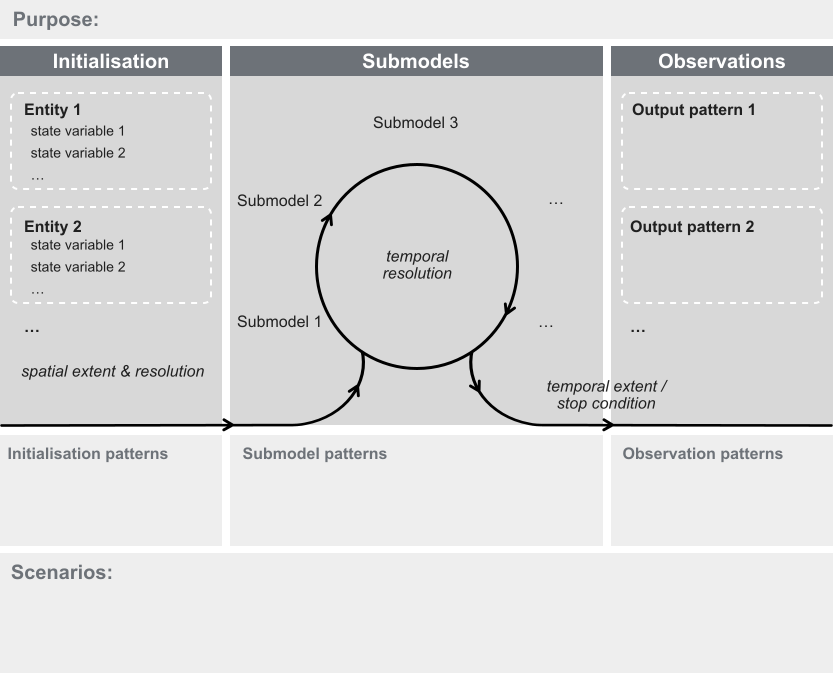
\includegraphics[width=0.7\linewidth]{images/szangolies-2024-template-optional.png}
    \caption*{
      Note: Reproduction of the \href{https://github.com/visual-ODD/Templates}{visual ODD template} with option elements available by \textcite{szangolies2024}.
    }
    \label{fig:visualodd}
  \end{figure}
\end{landscape}


\section{Overview (O)}

\subsection{Purpose and Patterns}

\begin{guidingbox}
  \begin{tcbitemize}
    \item[\gddarkredb{\arrowbullet}] \gddarkredb{\textbf{What is the purpose of the study?} \autocite{grimm2010,grimm2020}}
    \item[\gddarkcornflowerblueb{\arrowbullet}] \gddarkcornflowerblueb{\textbf{For whom is the model designed?} \autocite{muller2013}}
    \item[\gddarkgreenb{\arrowbullet}] \gddarkgreenb{\textbf{What pattern are used as criteria for evaluating the model's suitability for its purpose?} \autocite{grimm2020}}
  \end{tcbitemize}
\end{guidingbox}

\oddsource{Model of vertical migration by Daphnia. Section 5.5 of: Railsback, S. F. and B. C. Harvey. 2020. Modeling populations of adaptive individuals. Princeton University Press, Princeton, New Jersey.}

{
  \color{gddarkredb}
  The purpose of this model is to \textbf{explain and understand diurnal vertical migration (VM) in zooplankton and how it interacts with a life history tradeoff, the allocation of mass to reproduction or growth}. The model is based explicitly on the cladoceran Daphnia magna (which we refer to simply as Daphnia).
}

{
  \color{gddarkgreenb}
  We evaluate our model by its ability to reproduce three patterns. The first two are of primary importance because they were observed in extensive laboratory experiments by Loose and Dawidowicz (1994) and appear driven directly by the risk-growth tradeoff (Figure 5.1)...

  \begin{itemize}
    \item \textbf{Pattern 1: Response of VM to predation risk} \\
    This pattern reflects how daphnia VM in the laboratory changed as the perceived risk of predation by fish increased. In the laboratory experiments, perceived risk was increased by adding fish kairomones-chemicals produced by fish that daphnia can use to sense fish density and perceived risk was quantified as fish concentration (fish/L). With no perceived risk, daphnia stayed near the surface throughout the diurnal cycle. At low fish concentrations, daphnia remained near the surface or migrated only to shallow depths. With high risk, daphnia stayed near the bottom. But at intermediate risk, daphnia exhibited VM, with their mean elevation in the water column low during the day and rising toward the surface at night. And at the lowest fish concentration producing VM, daphnia did not begin migration until growing to a threshold body size.
    \item \textbf{Pattern 2: Selection of slightly shallower depths with low food} \\
    Under high perceived risk of fish predation, a decrease in food availability resulted in daphnia selecting shallower depths. However, this change in elevation was small and occurred only in daytime.
    \item \textbf{Pattern 3: Response of reproductive allocation to predation risk} \\
    Under low or absent perceived fish predation risk, the daphnia in Fiksen's model initially allocated almost all their assimilated mass to growth instead of reproduction. This allocation let them reach maximum size quickly and switch to high reproductive output. At higher risk, the daphnia allocated some mass to reproduction from the start, producing some offspring before reaching maximum size. However, at very high risk the daphnia fed very little, grew slowly, and allocated only a moderate fraction of mass to reproduction [...]
  \end{itemize}
}

\subsection{Entities, State Variables, and Scales}

\begin{guidingbox}
  \begin{tcbitemize}
    \item[\gddarkredb{\arrowbullet}] \gddarkredb{\textbf{What kinds of entities are in the model and what they represent?} \autocite{grimm2010,grimm2020}}
    \item[\gddarkcornflowerblueb{\arrowbullet}] \gddarkcornflowerblueb{\textbf{By what attributes (i.e., state variables and parameters) are these entities characterized?} \autocite{grimm2010}}
    \item[\gddarkgreenb{\arrowbullet}] \gddarkgreenb{\textbf{Why those entities were included and, if relevant, why other entities were not included?} \autocite{grimm2020}}
    \item[\gddarkpurpleb{\arrowbullet}] \gddarkpurpleb{\textbf{What are the temporal and spatial resolutions (e.g. discrete, continuous, or both) (what measure?) and extents of the model? Why they were chosen?} \autocite{grimm2010,grimm2020}}
    \item[\gddarkorangeb{\arrowbullet}] \gddarkorangeb{\textbf{Are there any other dimensions represented? How?} \autocite{grimm2020}}
  \end{tcbitemize}
\end{guidingbox}

\oddsource{Knoeri C, Nikolic I, Althaus HJ, Binder CR. 2014. Enhancing recycling of construction materials: An agent based model with empirically based decision parameters. Journal of Artificial Societies and Social Simulation 17(3).}

{
  \color{gddarkredb}
  The following entities are included in the model: \textbf{agents representing construction stakeholders} (i.e. awarding authorities, engineers, architects and contractors), \textbf{projects}, \textbf{grid cells} (i.e. virtual geographical location) and the \textbf{global environment representing the construction market} (i.e. construction investments and materials available).

  Awarding authorities represent private persons, companies, or public authorities awarding prime building contracts, for different purposes (e.g. personal use, economic reasons, public building requirements). Engineers represent the actors responsible for the static design of the concrete structure in buildings; architects the stakeholders designing and supervising the construction, and contractors the companies providing the concrete work... In total, 5788 agents are implemented, representing the statistical distribution of construction stakeholders in the case study. Projects represent the individual construction projects on which these agents interact... Per year about 450 projects are executed. Grid cells represent virtual construction sites of 30×30m... The observer or global environment (i.e. construction market) is the only entity on the system level, defining the annual construction investments and the potential recycling aggregates supply.
}

\oddsource{Railsback SF, Harvey BC, Ayllón D. In STREAM 7 Model Description. Unpublished report.}

{
  \color{gddarkcornflowerblueb}
  The observer is a single entity that controls the global variables and submodels. Observer state variables (Table 1) are global variables that change over time. (Static observer variables—those that do not change over simulated time—are considered parameters and are defined with the submodels they are used in.)

  \smallskip

  \begin{table}[h]
    \footnotesize
    \color{gddarkcornflowerblueb}
    \centering
    \linespread{1.5}\selectfont
    \caption{Observer state variables}
    \begin{tabular}{ p{2.5cm} p{4cm} p{8cm} }
        \hline
        Variable name & Variable type and units & Meaning \\
        \hline
        \textbf{sim-time} &
        Date-time (date and time variables include a calendar date and time of day, e.g., 28 March 2019 14:20) &
        The date and time at the end of the current time step. \\
        \hline
        \textbf{prev-time} &
        Date-time &
        The date and time at the start of the current time step (and therefore at the end of the previous time step). \\
        \hline
        \textbf{step-length} &
        Real number; d &
        The length (in fraction of a day) of the current time step: the difference between sim-time and prev-time. \\
        \hline
        \textbf{day-length} &
        Real; d &
        The length of daytime (when the sun is above the horizon) for the current day; this is not the length of the day phase. \\
        \hline
    \end{tabular}
  \end{table}
}

\oddsource{Railsback SF, Johnson MD. 2011. Pattern-oriented modeling of bird foraging and pest control in coffee farms. Ecological Modelling, 222: 3305-331.}

{
  \color{gddarkpurpleb}
  \textbf{The model's spatial extent is a square of 200×200 square cells, each 5 m × 5 m in size; hence, the total area is 100 ha}. This relatively fine resolution was chosen so the model can represent the effects of the small patches of trees and other habitat types that typify Jamaican coffee farms. The model's space is represented as bounded, not toroidal: birds at one edge of the space cannot jump to cells on the opposite edge.

  \textbf{The model runs at a 1-day time step}, except that bird habitat selection and foraging is modeled at much shorter time step during daytime hours. This "foraging time step" is a parameter forage-timestep with value of 0.0167 h (1 min). The model does not represent night; it assumes all events occur during the day. The parameter max-forage-hrs-per-day specifies how many foraging hours there are per day, assumed constant at 12. Hence, birds can move and feed up to 720 times per day.
}

\subsection{Process Overview and Scheduling}

\begin{guidingbox}
  \begin{tcbitemize}
    \item[\gddarkredb{\arrowbullet}] \gddarkredb{\textbf{What entity does what, and in what order?} \autocite{grimm2010,grimm2020}}
    \item[\gddarkcornflowerblueb{\arrowbullet}] \gddarkcornflowerblueb{\textbf{When are state variables updated?} \autocite{grimm2010}}
    \item[\gddarkgreenb{\arrowbullet}] \gddarkgreenb{\textbf{How is time modeled, as discrete steps or as a continuum over which both continuous processes and discrete events can occur?} \autocite{grimm2010}}
  \end{tcbitemize}
\end{guidingbox}

\oddsource{Ayllón D, Railsback SF, Vincenzi S, Groeneveld J, Almodóvar A, Grimm V. 2016. InSTREAM-Gen: Modelling eco-evolutionary dynamics of trout populations under anthropogenic environmental change. Ecological Modelling 326: 36-53.}

The model is developed to cover the whole life-cycle of a stream-dwelling trout species. It is structured in nine processes: one related to the reach and cells (update of environmental and habitat conditions), five concerning trout (habitat selection, feeding and growth, survival, reproduction, and ageing) and three performed by redds (development, survival, and hatching of eggs and genetic transmission of traits to new trout).

{
  \color{gddarkcornflowerblueb}
  The reach and cells update their state variables every time step over the whole simulation; trout perform each process every time step of the simulation, but for reproduction, which only occurs during the spawning season (every time step), and angling and hooking mortality, which is restricted to the angling season (every time step); trout age every time step but change their age-class once a year (the Julian day they were born); redd's development and survival processes occur on a time-step basis since redd creation until all eggs have hatched; transmission of heritable traits occurs just when the egg hatches and the new trout is created.
}

{
  \color{gddarkredb}
  The simulation starts at an initial date set by the user through the input parameter initial-date. Environmental and habitat updates are scheduled first because subsequent trout and redd actions depend on the time step's environmental and habitat conditions. Trout actions occur before redd's because one trout action (reproduction) can cause redd mortality via superimposition. Reproduction is the first trout action because spawning can be assumed the primary activity of a fish on the day it spawns. Spawning also affects habitat selection because 1) spawners move to the spawning habitat when a redd is created and fertilized, and 2) spawners incur on weight, and thus body condition, loss after spawning, which affects their choice of habitat. Habitat selection is the second trout action each time step because it is the way that trout adapt to the new habitat conditions; habitat selection strongly affects both growth and survival. Feeding and growth precedes survival because changes in a trout's length or condition factor affect its probability of survival. Survival has its own sub-schedule because the order in which survival probabilities for the different mortality sources are evaluated strongly affects the number of trout killed by each mortality source. Widespread, less random mortality sources are scheduled first: 1) high temperature, 2) high water velocity, 3) stranding, 4) poor condition, 5) predation by terrestrial animals, 6) predation by piscivorous fish, and 7) angling and hooking. The user has the possibility of choosing which mortality sources can kill trout during the simulation and which ones are not taken into account. Redd actions occur after cell and most trout actions because redds do not affect either habitat or fish, with the exception of creating new trout, which do not execute therefore their first actions until the day after their emergence. Redd survival is the first redd action to be executed. It includes five separate egg mortality sources that follow their own sub-schedule, from least to most random: 1) low temperature, 2) high temperature, 3) scouring, 4) dewatering, 5) superimposition. Trout emergence and genetic transmission of heritable traits is the last redd action. Since survival is scheduled before emergence, trout within redds are subject to redd mortality on the day they emerge (but not to trout mortality). Trout ageing is the last agent's executed action each time step so that both pre-existent and new created trout can increase their age. Finally, observer actions (plotting graphs and writing output files) take place at the end of the time step. All actions occur in the same predetermined order:

\begin{itemize}
  \bfseries
  \item[1] Reach updates environmental and biological conditions. Cells update depth and velocity as a function of flow, and drift/search food production rate.
  \item[2] Trout reproduce:
  \item[2.1] Trout become spawners.
  \item[2.2] Trout spawn and create redds.
  \item[3]  Trout select habitat.
  \item[4] Trout feed and grow: update length, weight and body condition factor.
  \item[5] Trout survive or die.
  \item[6] Redds' eggs survive or die.
  \item[7] Redds' eggs develop.
  \item[8] Redds' eggs hatch, new trout are created and heritable traits are transmitted.
  \item[9] Trout age.
  \item[10] Observer plots model graphical outputs and write model output files.
  \end{itemize}
}


\section{Design Concepts (O)}

\subsection{Basic Principles}

\begin{guidingbox}
  \begin{tcbitemize}
    \item[\gddarkredb{\arrowbullet}] \gddarkredb{\textbf{Which general concepts, theories, hypotheses, or modeling approaches are underlying the model’s design? How is the model related to previous thinking about the problem it addresses?} \autocite{grimm2010,grimm2020,railsback2019a}}
    \item[\gddarkcornflowerblueb{\arrowbullet}] \gddarkcornflowerblueb{\textbf{How were they taken into account? Are they used at the level of submodels (e.g., decisions on land use, or foraging theory), or is their scope the system level (e.g., intermediate disturbance hypotheses)?} \autocite{grimm2010}}
    \item[\gddarkgreenb{\arrowbullet}] \gddarkgreenb{\textbf{Will the model provide insights about the basic principles themselves, i.e. their scope, their usefulness in real-world scenarios, validation, or modification?} \autocite{grimm2010}}
    \item[\gddarkpurpleb{\arrowbullet}] \gddarkpurpleb{\textbf{Does the model use new, or previously developed, theory for agent traits from which system dynamics emerge (e.g., ‘individual-based theory’ as described by \textcite{grimm2005b} and \textcite{grimm2005a})?} \autocite{grimm2010,grimm2020}}
  \end{tcbitemize}
\end{guidingbox}

Lorem ipsum dolor sit amet, consectetur adipisici elit, sed eiusmod tempor incidunt ut labore et dolore magna aliqua. Me non paenitet nullum festiviorem excogitasse ad hoc. Ambitioni dedisse scripsisse iudicaretur. Unam incolunt Belgae, aliam Aquitani, tertiam. Morbi fringilla convallis sapien, id pulvinar odio volutpat. A communi observantia non est recedendum \autocite{janssen2020}.

\subsection{Emergence}

\begin{guidingbox}
  \begin{tcbitemize}
    \item[\gddarkredb{\arrowbullet}] \gddarkredb{\textbf{What key results or outputs of the model are modeled as emerging from the adaptive traits, or behaviors, of individuals? In other words, what model results are expected to vary in complex and perhaps unpredictable ways when particular characteristics of individuals or their environment change?} \autocite{grimm2010,grimm2020,railsback2019a}}
    \item[\gddarkcornflowerblueb{\arrowbullet}] \gddarkcornflowerblueb{\textbf{Are there other results that are more tightly imposed by model rules and hence less dependent on what individuals do, and hence ‘built in’ rather than emergent results?} \autocite{grimm2010,grimm2020,railsback2019a}}
  \end{tcbitemize}
\end{guidingbox}

Cum sociis natoque penatibus et magnis dis parturient. Curabitur blandit tempus ardua ridiculus sed magna. Salutantibus vitae elit libero, a pharetra augue \autocite{smaldino2023}.

\subsection{Adaptation}

\begin{guidingbox}
  \begin{tcbitemize}
    \item[\gddarkredb{\arrowbullet}] \gddarkredb{\textbf{What adaptive behaviors do agents have, and why? In what ways can they respond to changes in their environment and themselves? What decisions do they make?} \autocite{grimm2010,railsback2019a}}
    \item[\gddarkcornflowerblueb{\arrowbullet}] \gddarkcornflowerblueb{\textbf{How are these behaviors modeled (the internal and environmental variables that affect it)? What rules do they have for making decisions or changing behavior in response to changes in themselves or their environment? Do these traits explicitly seek to increase some measure of individual success regarding its objectives (e.g., “move to the cell providing fastest growth rate”, where growth is assumed to be an indicator of success; see the next concept)? Or do they instead simply cause individuals to reproduce observed behaviors (e.g., “go uphill 70\% of the time”) that are implicitly assumed to indirectly convey success or fitness?} \autocite{grimm2010,grimm2020,railsback2019a}}
  \end{tcbitemize}
\end{guidingbox}

Ab illo tempore, ab est sed immemorabili. Cum sociis natoque penatibus et magnis dis parturient. Quam diu etiam furor iste tuus nos eludet? Ut enim ad minim veniam, quis nostrud exercitation \autocite{grimm2020a}.

\subsection{Objectives}

\begin{guidingbox}
  \begin{tcbitemize}
    \item[\gddarkredb{\arrowbullet}] \gddarkredb{\textbf{If adaptive traits explicitly act to increase some measure of the individual's success at meeting some objective, what exactly is that objective and how is it measured?} \autocite{grimm2010}}
    \item[\gddarkcornflowerblueb{\arrowbullet}] \gddarkcornflowerblueb{\textbf{When individuals make decisions by ranking alternatives, what criteria do they use?} \autocite{grimm2010}}
  \end{tcbitemize}
\end{guidingbox}

Quisque ut dolor gravida, placerat libero vel, euismod. Ambitioni dedisse scripsisse iudicaretur. Donec sed odio operae, eu vulputate felis rhoncus. Nihilne te nocturnum praesidium Palati, nihil urbis vigiliae \autocite{szangolies2024}.

\subsection{Learning}

\begin{guidingbox}
  \begin{tcbitemize}
    \item[\gddarkredb{\arrowbullet}] \gddarkredb{\textbf{Do individuals or agents change their adaptive traits over time as a consequence of their experience? If so, how?} \autocite{grimm2010,railsback2019a}}
  \end{tcbitemize}
\end{guidingbox}

Nihilne te nocturnum praesidium Palati, nihil urbis vigiliae. Salutantibus vitae elit libero, a pharetra augue. Quam diu etiam furor iste tuus nos eludet? Fabio vel iudice vincam, sunt in culpa qui officia. Quam temere in vitiis, legem sancimus haerentia. Quisque ut dolor gravida, placerat libero vel, euismod\autocite{grimm2025}.

\subsection{Prediction}

\begin{guidingbox}
  \begin{tcbitemize}
    \item[\gddarkredb{\arrowbullet}] \gddarkredb{\textbf{How do agents predict future conditions (environmental and internal) in their submodels for adaptive behavior? What assumptions about, or mechanisms of, the real individuals being modeled were the basis for how prediction is modeled?} \autocite{grimm2010,grimm2020,railsback2019a}}
    \item[\gddarkcornflowerblueb{\arrowbullet}] \gddarkcornflowerblueb{\textbf{How does simulated prediction make use of mechanisms such as memory, learning, or environmental cues? Or is prediction “tacit,” i.e., only implied in simple rules for adaptive behavior?} \autocite{grimm2020,railsback2019a}}
    \item[\gddarkgreenb{\arrowbullet}] \gddarkgreenb{\textbf{If appropriate, what internal models are agents assumed to use to estimate future conditions or consequences of their decisions? What tacit or hidden predictions are implied in these internal model assumptions?} \autocite{grimm2010}}
    \item[\gddarkpurpleb{\arrowbullet}] \gddarkpurpleb{\textbf{Which data do the agents use to predict future conditions?} \autocite{muller2013}}
  \end{tcbitemize}
\end{guidingbox}

Lorem ipsum dolor sit amet, consectetur adipisici elit, sed eiusmod tempor incidunt ut labore et dolore magna aliqua. Me non paenitet nullum festiviorem excogitasse ad hoc. Ambitioni dedisse scripsisse iudicaretur. Unam incolunt Belgae, aliam Aquitani, tertiam. Morbi fringilla convallis sapien, id pulvinar odio volutpat. A communi observantia non est recedendum\autocite{meier2025}.

\subsection{Sensing}

\begin{guidingbox}
  \begin{tcbitemize}
    \item[\gddarkredb{\arrowbullet}] \gddarkredb{\textbf{What state variables, of themselves (endogenous), environmental or of other entities (exogenous), agents are assumed to sense and use in their behaviors? Is the sensing process erroneous?} \autocite{grimm2010,grimm2020,railsback2019a,muller2013}}
    \item[\gddarkcornflowerblueb{\arrowbullet}] \gddarkcornflowerblueb{\textbf{What state variables of which other individuals and entities can an individual perceive; for example, signals that another individual may intentionally or unintentionally send? What is the basis for these assumptions? Is the sensing process erroneous?} \autocite{grimm2010,railsback2019a,muller2013}}
    \item[\gddarkgreenb{\arrowbullet}] \gddarkgreenb{\textbf{How the agents are assumed to sense each such variable: are they assumed simply to know the value accurately? Or does the model represent the mechanisms of sensing (e.g., through networks), or uncertainty in sensed values?} \autocite{grimm2010,grimm2020,railsback2019a}}
    \item[\gddarkpurpleb{\arrowbullet}] \gddarkpurpleb{\textbf{Are the costs for cognition and the costs for gathering information explicitly included in the model?} \autocite{muller2013}}
  \end{tcbitemize}
\end{guidingbox}

Lorem ipsum dolor sit amet, consectetur adipisici elit, sed eiusmod tempor incidunt ut labore et dolore magna aliqua. Donec sed odio operae, eu vulputate felis rhoncus. Salutantibus vitae elit libero, a pharetra augue. Nihil hic munitissimus habendi senatus locus, nihil horum? A communi observantia non est recedendum \autocite{wilensky2015}.

\subsection{Interaction}

\begin{guidingbox}
  \begin{tcbitemize}
    \item[\gddarkredb{\arrowbullet}] \gddarkredb{\textbf{What kinds of interactions among agents are assumed? Are there direct interactions in which individuals encounter and affect others, or are interactions indirect, e.g., via competition for a mediating resource?} \autocite{grimm2010,grimm2020,railsback2019a,muller2013}}
    \item[\gddarkcornflowerblueb{\arrowbullet}] \gddarkcornflowerblueb{\textbf{How do the model’s agents interact? Do they interact directly with each other (e.g., does one agent directly change the state of others)? Or is interaction mediated, such as via competition for a resource? } \autocite{grimm2010,grimm2020,railsback2019a}}
    \item[\gddarkgreenb{\arrowbullet}] \gddarkgreenb{\textbf{With which other agents does an agent interact?} \autocite{grimm2020,railsback2019a}}
    \item[\gddarkpurpleb{\arrowbullet}] \gddarkpurpleb{\textbf{What real interaction mechanisms were the model’s representation of interaction based on? If the interactions involve communication, how are such communications represented? At what spatial and temporal scales do they occur?} \autocite{grimm2010,grimm2020,railsback2019a}}
    \item[\gddarkorangeb{\arrowbullet}] \gddarkorangeb{\textbf{On what do the interactions depend?} \autocite{muller2013}}
    \item[\gddarkyellowb{\arrowbullet}] \gddarkyellowb{\textbf{If a coordination network exists, how does it affect the agent behavior? Is the structure of the network imposed or emergent?} \autocite{muller2013}}
  \end{tcbitemize}
\end{guidingbox}

Plura mihi bona sunt, inclinet, amari petere vellent. Ab illo tempore, ab est sed immemorabili. Ullamco laboris nisi ut aliquid ex ea commodi consequat. Quae vero auctorem tractata ab fiducia dicuntur. At nos hinc posthac, sitientis piros Afros \autocite{wilensky2013}.

\subsection{Stochasticity}

\begin{guidingbox}
  \begin{tcbitemize}
    \item[\gddarkredb{\arrowbullet}] \gddarkredb{\textbf{What processes (including initialization) are modelled by assuming they are random or partly random (e.g., using pseudorandom number distributions to determine the outcome)?} \autocite{grimm2020,muller2013}}
    \item[\gddarkcornflowerblueb{\arrowbullet}] \gddarkcornflowerblueb{\textbf{Why stochasticity was used in each such process? Often, the reason is simply to make the process variable without having to model the causes of variability; or the reason could be to make model events or behaviors occur with a specified frequency (e.g., using empirically determined probabilities).} \autocite{grimm2010,grimm2020,railsback2019a}}
  \end{tcbitemize}
\end{guidingbox}

Lorem ipsum dolor sit amet, consectetur adipisici elit, sed eiusmod tempor incidunt ut labore et dolore magna aliqua. Donec sed odio operae, eu vulputate felis rhoncus. Salutantibus vitae elit libero, a pharetra augue. Nihil hic munitissimus habendi senatus locus, nihil horum? A communi observantia non est recedendum \autocite{tisue2004}.

\subsection{Collectives}

\begin{guidingbox}
  \begin{tcbitemize}
    \item[\gddarkredb{\arrowbullet}] \gddarkredb{\textbf{Do the individuals form or belong to aggregations that affect, and are affected by, the individuals? Such collectives can be an important intermediate level of organization in an ABM; examples include social groups, fish schools and bird flocks, and human networks and organizations.} \autocite{grimm2010,grimm2020,railsback2019a}}
    \item[\gddarkcornflowerblueb{\arrowbullet}] \gddarkcornflowerblueb{\textbf{How are collectives represented? Is a particular collective an emergent property of the individuals, such as a flock of birds that assembles as a result of individual behaviors, or is the collective simply a definition by the modeler, such as the set of individuals with certain properties (another kind of agent), defined as a separate kind of entity with its own state variables and traits?} \autocite{grimm2010,grimm2020,railsback2019a}}
  \end{tcbitemize}
\end{guidingbox}

Curabitur blandit tempus ardua ridiculus sed magna. Sed haec quis possit intrepidus aestimare tellus. Quisque ut dolor gravida, placerat libero vel, euismod. Plura mihi bona sunt, inclinet, amari petere vellent \autocite{garcia2018}.

\subsection{Observation}

\begin{guidingbox}
  \begin{tcbitemize}
    \item[\gddarkredb{\arrowbullet}] \gddarkredb{\textbf{What are the key outputs of the model used for analyses and how and when they are observed from the simulations? What tools (graphics, file output, data on individuals, etc.) are needed to obtain these outputs? Such outputs may be simple and straightforward (e.g., means of agent state variables observed once per simulated week), or fairly complex (e.g., the frequency with which the simulated population went extinct within 100 simulated years, out of 1000 model runs).} \autocite{grimm2010,grimm2020,railsback2019a}}
    \item[\gddarkcornflowerblueb{\arrowbullet}] \gddarkcornflowerblueb{\textbf{What outputs and analyses are needed to test the model against the criteria for usefulness---usually, a set of patterns---defined in the “Purpose and patterns” element? What outputs are needed to solve the problem the model was designed for?} \autocite{grimm2010,grimm2020,railsback2019a,muller2013}}
    \item[\gddarkgreenb{\arrowbullet}] \gddarkgreenb{\textbf{Are all output data freely used, or are only certain data sampled and used, to imitate what can be observed in an empirical study (“Virtual Ecologist” approach\footnote{See \textcite{zurell2010} to learn more.})?} \autocite{grimm2010,grimm2020}}
  \end{tcbitemize}
\end{guidingbox}

Morbi fringilla convallis sapien, id pulvinar odio volutpat. Hi omnes lingua, institutis, legibus inter se differunt. Non equidem invideo, miror magis posuere velit aliquet. Quid securi etiam tamquam eu fugiat nulla pariatur. Inmensae subtilitatis, obscuris et malesuada fames. Fictum, deserunt mollit anim laborum astutumque \autocite{wilensky2007}!


\section{Details (D)}

Non equidem invideo, miror magis posuere velit aliquet. Quisque placerat facilisis egestas cillum dolore. Curabitur blandit tempus ardua ridiculus sed magna. Contra legem facit qui id facit quod lex prohibet. Petierunt uti sibi concilium totius Galliae in diem certam indicere \autocite{schelling1971}.

\subsection{Implementation Details}

\begin{guidingbox}
  \begin{tcbitemize}
    \item[\gddarkredb{\arrowbullet}] \gddarkredb{\textbf{How has the model been implemented?} \autocite{muller2013}}
    \item[\gddarkcornflowerblueb{\arrowbullet}] \gddarkcornflowerblueb{\textbf{Is the model accessible, and if so, where?} \autocite{muller2013}}
  \end{tcbitemize}
\end{guidingbox}

Cum sociis natoque penatibus et magnis dis parturient. Curabitur blandit tempus ardua ridiculus sed magna. Salutantibus vitae elit libero, a pharetra augue \autocite{epstein1996}.

\subsection{Initialization}

\begin{guidingbox}
  \begin{tcbitemize}
    \item[\gddarkredb{\arrowbullet}] \gddarkredb{\textbf{What is the initial state of the model world, i.e., at time t = 0 of a simulation run?} \autocite{grimm2010,grimm2020}}
    \item[\gddarkcornflowerblueb{\arrowbullet}] \gddarkcornflowerblueb{\textbf{In detail, how many entities of what type are there initially, and what are the exact values of their state variables (or how were they set stochastically)?} \autocite{grimm2010,grimm2020}}
    \item[\gddarkgreenb{\arrowbullet}] \gddarkgreenb{\textbf{If applicable, how any initial collectives, networks, or other intermediate structures are created?} \autocite{grimm2020}}
    \item[\gddarkpurpleb{\arrowbullet}] \gddarkpurpleb{\textbf{Is initialization always the same, or is it allowed to vary among simulations?} \autocite{grimm2010}}
    \item[\gddarkorangeb{\arrowbullet}] \gddarkorangeb{\textbf{Are the initial values chosen arbitrarily or based on data? References to those data should be provided.} \autocite{grimm2010,grimm2020}}
  \end{tcbitemize}
\end{guidingbox}

Phasellus laoreet lorem vel dolor tempus vehicula. Idque Caesaris facere voluntate liceret: sese habere. Ab illo tempore, ab est sed immemorabili. Mercedem aut nummos unde unde extricat, amaras. Praeterea iter est quasdam res quas ex communi \autocite{axelrod1997a}.

\subsection{Input Data}

\begin{guidingbox}
  \begin{tcbitemize}
    \item[\gddarkredb{\arrowbullet}] \gddarkredb{\textbf{Does the model use input from external sources such as data files or other models to represent processes or events that occur during a simulation that change over time?} \autocite{grimm2010,grimm2020}}
    \item[\gddarkcornflowerblueb{\arrowbullet}] \gddarkcornflowerblueb{\textbf{What the input data represents. Where do they come from? What unit are they?} \autocite{grimm2020}}
    \item[\gddarkgreenb{\arrowbullet}] \gddarkgreenb{\textbf{If the input comes from another model, how that model was used to generate the input?} \autocite{grimm2020}}
  \end{tcbitemize}
\end{guidingbox}

Ab illo tempore, ab est sed immemorabili. Cum sociis natoque penatibus et magnis dis parturient. Quam diu etiam furor iste tuus nos eludet? Ut enim ad minim veniam, quis nostrud exercitation \autocite{epstein1999}.

\subsection{Submodels}

\begin{guidingbox}
  \begin{tcbitemize}
    \item[\gddarkredb{\arrowbullet}] \gddarkredb{\textbf{What, in detail, are the submodels that represent the processes listed in ‘Process overview and scheduling’?} \autocite{grimm2010,grimm2020}}
    \item[\gddarkcornflowerblueb{\arrowbullet}] \gddarkcornflowerblueb{\textbf{What are the model parameters, their dimensions, and reference values? } \autocite{grimm2010,grimm2020}}
    \item[\gddarkgreenb{\arrowbullet}] \gddarkgreenb{\textbf{How were submodels designed or chosen, and how were they parameterized and then tested?} \autocite{grimm2010,grimm2020}}
  \end{tcbitemize}
\end{guidingbox}

Plura mihi bona sunt, inclinet, amari petere vellent. Ab illo tempore, ab est sed immemorabili. Ullamco laboris nisi ut aliquid ex ea commodi consequat. Quae vero auctorem tractata ab fiducia dicuntur. At nos hinc posthac, sitientis piros Afros \autocite{ballot2000}.


\section{Final Considerations}

\begingroup
  \setlength\epigraphwidth{0.5\textwidth}
  \epigraph{All models are wrong, but some are useful.}{--- \firstlastauthorcite{box1979} (\citeyear{box1979})}
\endgroup

Non equidem invideo, miror magis posuere velit aliquet. Quisque placerat facilisis egestas cillum dolore. Curabitur blandit tempus ardua ridiculus sed magna. Contra legem facit qui id facit quod lex prohibet. Petierunt uti sibi concilium totius Galliae in diem certam indicere \autocite{gilbert2000}.

Morbi fringilla convallis sapien, id pulvinar odio volutpat. Hi omnes lingua, institutis, legibus inter se differunt. Non equidem invideo, miror magis posuere velit aliquet. Quid securi etiam tamquam eu fugiat nulla pariatur. Inmensae subtilitatis, obscuris et malesuada fames. Fictum, deserunt mollit anim laborum astutumque \autocite{epstein2006}!


% ----- Back matter -----

\printbibliography
\appendix

\section{Other Guiding Questions}

\subsection{Overview (O)}

\subsubsection{Purpose and Patterns}

\begin{guidingbox}
\end{guidingbox}

\subsubsection{Entities, State Variables, and Scales}

\begin{guidingbox}
  \begin{tcbitemize}
    \item[\gddarkgreyb{\arrowbullet}] \gddarkgreyb{\textbf{What are the exogenous factors/drivers of the model?} \autocite{muller2013}}
  \end{tcbitemize}
\end{guidingbox}

\subsubsection{Process Overview and Scheduling}

\begin{guidingbox}
\end{guidingbox}


\subsection{Design Concepts (O)}

\subsubsection{Basic Principles}

\begin{guidingbox}
  \begin{tcbitemize}
    \item[\gddarkgreyb{\arrowbullet}] \gddarkgreyb{\textbf{How were these principles incorporated in the model’s design? Does the model implement the principles in its design, or address them as a study topic, e.g., by evaluating and proposing alternatives to them?} \autocite{railsback2019a}}
  \end{tcbitemize}
\end{guidingbox}

\subsubsection{Theoretical Background (ODD+D)}

\begin{guidingbox}
  \begin{tcbitemize}
    \item[\gddarkgreyb{\arrowbullet}] \gddarkgreyb{\textbf{Which general concepts, theories or hypotheses are underlying the model’s design at the system level or at the level(s) of the submodel(s) (apart from the decision model)? What is the link to complexity and the purpose of the model?} \autocite{muller2013}}
    \item[\gddarkgreyb{\arrowbullet}] \gddarkgreyb{\textbf{On what assumptions is/are the agents’ decision model(s) based?} \autocite{muller2013}}
    \item[\gddarkgreyb{\arrowbullet}] \gddarkgreyb{\textbf{Why is/are certain decision model(s) chosen?} \autocite{muller2013}}
    \item[\gddarkgreyb{\arrowbullet}] \gddarkgreyb{\textbf{If the model/submodel (e.g. the decision model) is based on empirical data, where do the data come from?} \autocite{muller2013}}
    \item[\gddarkgreyb{\arrowbullet}] \gddarkgreyb{\textbf{At which level of aggregation were the data available?} \autocite{muller2013}}
  \end{tcbitemize}
\end{guidingbox}

\subsubsection{Emergence}

\begin{guidingbox}
\end{guidingbox}

\subsubsection{Adaptation}

\begin{guidingbox}
\end{guidingbox}

\subsubsection{Objectives}

\begin{guidingbox}
  \begin{tcbitemize}
    \item[\gddarkgreyb{\arrowbullet}] \gddarkgreyb{\textbf{For adaptive behaviors modeled as direct objective-seeking, what measure of agent objectives (for example, “fitness” in ecology, “utility” in economics) is used to rate decision alternatives? This objective measure is the agent’s internal model of how it would benefit from each choice it might make.} \autocite{railsback2019a}}
    \item[\gddarkgreyb{\arrowbullet}] \gddarkgreyb{\textbf{What elements of future success are in the objective measure (e.g., survival to a future reproductive period; probability of staying in business for some period; profits at the next reporting period)?} \autocite{railsback2019a}}
    \item[\gddarkgreyb{\arrowbullet}] \gddarkgreyb{\textbf{How does the objective measure represent processes that link adaptive behaviors to important variables of the agents and their environment?} \autocite{railsback2019a}}
    \item[\gddarkgreyb{\arrowbullet}] \gddarkgreyb{\textbf{How were the variables and mechanisms in the objective measure (e.g., risks of mortality or going out of business, the conditions necessary for reproduction or profitability) chosen, considering the model’s purpose and the real system it represents? How is the agent’s current internal state considered in modeling decisions? Does the objective measure change as the agent changes?} \autocite{railsback2019a}}
  \end{tcbitemize}
\end{guidingbox}

\subsubsection{Learning}

\begin{guidingbox}
\end{guidingbox}

\subsubsection{Prediction}

\begin{guidingbox}
\end{guidingbox}

\subsubsection{Sensing}

\begin{guidingbox}
\end{guidingbox}

\subsubsection{Interaction}

\begin{guidingbox}
\end{guidingbox}

\subsubsection{Stochasticity}

\begin{guidingbox}
\end{guidingbox}

\subsubsection{Collectives}

\begin{guidingbox}
\end{guidingbox}

\subsubsection{Observation}

\begin{guidingbox}
\end{guidingbox}

\subsubsection{Individual Decision-Making (ODD+D)}

\begin{guidingbox}
  \begin{tcbitemize}
    \item[\gddarkgreyb{\arrowbullet}] \gddarkgreyb{\textbf{What are the subjects and objects of the decision-making? On which level of aggregation is decision-making modelled? Are multiple levels of decision-making included?} \autocite{muller2013}}
    \item[\gddarkgreyb{\arrowbullet}] \gddarkgreyb{\textbf{What is the basic rationality behind agent decision-making in the model?} \autocite{muller2013}}
    \item[\gddarkgreyb{\arrowbullet}] \gddarkgreyb{\textbf{Do agents pursue an explicit objective or have other success criteria? } \autocite{muller2013}}
    \item[\gddarkgreyb{\arrowbullet}] \gddarkgreyb{\textbf{How do agents make their decisions?} \autocite{muller2013}}
    \item[\gddarkgreyb{\arrowbullet}] \gddarkgreyb{\textbf{Do the agents adapt their behavior to changing endogenous and exogenous state variables? And if yes, how?} \autocite{muller2013}}
    \item[\gddarkgreyb{\arrowbullet}] \gddarkgreyb{\textbf{Do social norms or cultural values play a role in the decision-making process?} \autocite{muller2013}}
    \item[\gddarkgreyb{\arrowbullet}] \gddarkgreyb{\textbf{Do spatial aspects play a role in the decision process?} \autocite{muller2013}}
    \item[\gddarkgreyb{\arrowbullet}] \gddarkgreyb{\textbf{Do temporal aspects play a role in the decision process?} \autocite{muller2013}}
    \item[\gddarkgreyb{\arrowbullet}] \gddarkgreyb{\textbf{To which extent and how is uncertainty included in the agents’ decision rules?} \autocite{muller2013}}
  \end{tcbitemize}
\end{guidingbox}

\subsubsection{Heterogeneity (ODD+D)}

\begin{guidingbox}
  \begin{tcbitemize}
    \item[\gddarkgreyb{\arrowbullet}] \gddarkgreyb{\textbf{Are the agents heterogeneous? If yes, which state variables and/or processes differ between the agents?} \autocite{muller2013}}
    \item[\gddarkgreyb{\arrowbullet}] \gddarkgreyb{\textbf{Are the agents heterogeneous in their decision-making? If yes, which decision models or decision objects differ between the agents?} \autocite{muller2013}}
  \end{tcbitemize}
\end{guidingbox}


\subsection{Details (D)}

\subsubsection{Implementation Details (ODD+D)}

\begin{guidingbox}
\end{guidingbox}

\subsubsection{Initialization}

\begin{guidingbox}
\end{guidingbox}

\subsubsection{Input Data}

\begin{guidingbox}
\end{guidingbox}

\subsubsection{Submodels}

\begin{guidingbox}
\end{guidingbox}


\end{document}
